\documentclass{article}

\PassOptionsToPackage{numbers, compress}{natbib}
\usepackage[sglblindworkshop, final]{neurips_2026}
\workshoptitle{Predictive AI Evaluation Competition (PAIEC)}

\usepackage[utf8]{inputenc}
\usepackage[T1]{fontenc}
\usepackage{hyperref}
\usepackage{url}
\usepackage{booktabs}
\usepackage{amsmath,amssymb,amsfonts}
\usepackage{nicefrac}
\usepackage{microtype}
\usepackage{xcolor}
\usepackage{graphicx}
\usepackage{multirow}
\usepackage{makecell}
\usepackage{float}
\usepackage{needspace}
\usepackage[capitalise,noabbrev]{cleveref}

\definecolor{accent}{HTML}{2A78D6}
\hypersetup{colorlinks=true, linkcolor=accent, citecolor=accent, urlcolor=accent,
  pdftitle={Items Are Shared, Abilities Are Not: Predicting AI Correctness on Unseen Benchmarks from Other Systems' Labels},
  pdfauthor={Vaibhav Kanojia}}
\newcommand{\ALC}{\mathrm{ALC}}
\newcommand{\Lb}{\mathcal{L}}
\DeclareMathOperator{\logit}{logit}
% Generated by paper/scripts/analyze_r7.py -- do not edit by hand.
\newcommand{\nStd}{1{,}738}
\newcommand{\nbStd}{144}
\newcommand{\aStdConst}{0.2500}
\newcommand{\ciStdConst}{[0.2500, 0.2500]}
\newcommand{\aStdEM}{0.2455}
\newcommand{\ciStdEM}{[0.2325, 0.2578]}
\newcommand{\aStdBeta}{0.2119}
\newcommand{\ciStdBeta}{[0.2028, 0.2204]}
\newcommand{\aStdEB}{0.2077}
\newcommand{\ciStdEB}{[0.1971, 0.2176]}
\newcommand{\aStdHier}{0.1991}
\newcommand{\ciStdHier}{[0.1896, 0.2079]}
\newcommand{\aStdHierU}{0.1984}
\newcommand{\ciStdHierU}{[0.1888, 0.2072]}
\newcommand{\aStdTok}{0.1950}
\newcommand{\ciStdTok}{[0.1854, 0.2039]}
\newcommand{\aStdTokRand}{0.1957}
\newcommand{\ciStdTokRand}{[0.1861, 0.2047]}
\newcommand{\aStdSix}{0.1945}
\newcommand{\ciStdSix}{[0.1849, 0.2034]}
\newcommand{\aStdSev}{0.1945}
\newcommand{\ciStdSev}{[0.1849, 0.2034]}
\newcommand{\aStdGate}{0.1942}
\newcommand{\ciStdGate}{[0.1846, 0.2031]}
\newcommand{\dStdUnc}{$-$0.0007}
\newcommand{\pStdUnc}{0.0007}
\newcommand{\pciStdUnc}{[$-$0.0002, 0.0015]}
\newcommand{\dciStdUnc}{[$-$0.0015, $+$0.0002]}
\newcommand{\dStdTokens}{$-$0.0034}
\newcommand{\pStdTokens}{0.0034}
\newcommand{\pciStdTokens}{[0.0023, 0.0046]}
\newcommand{\dciStdTokens}{[$-$0.0046, $-$0.0023]}
\newcommand{\dStdCov}{$-$0.0005}
\newcommand{\pStdCov}{0.0005}
\newcommand{\pciStdCov}{[0.0002, 0.0008]}
\newcommand{\dciStdCov}{[$-$0.0008, $-$0.0002]}
\newcommand{\dStdName}{$+$0.00001}
\newcommand{\pStdName}{-0.0000}
\newcommand{\pciStdName}{[$-$0.0004, 0.0003]}
\newcommand{\dciStdName}{[$-$0.0003, $+$0.0004]}
\newcommand{\dStdAct}{$-$0.0013}
\newcommand{\pStdAct}{0.0013}
\newcommand{\pciStdAct}{[0.0003, 0.0022]}
\newcommand{\dciStdAct}{[$-$0.0022, $-$0.0003]}
\newcommand{\dStdVsEM}{$-$0.0511}
\newcommand{\pStdVsEM}{0.0511}
\newcommand{\pciStdVsEM}{[0.0467, 0.0554]}
\newcommand{\dciStdVsEM}{[$-$0.0554, $-$0.0467]}
\newcommand{\dStdVsBeta}{$-$0.0174}
\newcommand{\pStdVsBeta}{0.0174}
\newcommand{\pciStdVsBeta}{[0.0153, 0.0198]}
\newcommand{\dciStdVsBeta}{[$-$0.0198, $-$0.0153]}
\newcommand{\dStdVsEB}{$-$0.0133}
\newcommand{\pStdVsEB}{0.0133}
\newcommand{\pciStdVsEB}{[0.0110, 0.0157]}
\newcommand{\dciStdVsEB}{[$-$0.0157, $-$0.0110]}
\newcommand{\dStdVsHier}{$-$0.0046}
\newcommand{\pStdVsHier}{0.0046}
\newcommand{\pciStdVsHier}{[0.0031, 0.0061]}
\newcommand{\dciStdVsHier}{[$-$0.0061, $-$0.0031]}
\newcommand{\dStdGate}{$-$0.0003}
\newcommand{\pStdGate}{0.0003}
\newcommand{\pciStdGate}{[$-$0.0001, 0.0007]}
\newcommand{\dciStdGate}{[$-$0.0007, $+$0.00010]}
\newcommand{\dStdSixVsBeta}{$-$0.0175}
\newcommand{\pStdSixVsBeta}{0.0175}
\newcommand{\pciStdSixVsBeta}{[0.0153, 0.0197]}
\newcommand{\dciStdSixVsBeta}{[$-$0.0197, $-$0.0153]}
\newcommand{\dStdSixVsEM}{$-$0.0511}
\newcommand{\pStdSixVsEM}{0.0511}
\newcommand{\pciStdSixVsEM}{[0.0467, 0.0554]}
\newcommand{\dciStdSixVsEM}{[$-$0.0554, $-$0.0467]}
\newcommand{\dStdSixVsEB}{$-$0.0133}
\newcommand{\pStdSixVsEB}{0.0133}
\newcommand{\pciStdSixVsEB}{[0.0111, 0.0156]}
\newcommand{\dciStdSixVsEB}{[$-$0.0156, $-$0.0111]}
\newcommand{\dStdNameKnown}{$-$0.0001}
\newcommand{\dciStdNameKnown}{[$-$0.0008, $+$0.0005]}
\newcommand{\nStdNameKnown}{795}
\newcommand{\dStdNameUnknown}{$+$0.0001}
\newcommand{\dciStdNameUnknown}{[$-$0.0001, $+$0.0004]}
\newcommand{\nStdNameUnknown}{943}
\newcommand{\relStdEM}{20.8}
\newcommand{\relSixStdEM}{20.8}
\newcommand{\relSixStdBeta}{8.2}
\newcommand{\relStdBeta}{8.2}
\newcommand{\nHigh}{891}
\newcommand{\nbHigh}{113}
\newcommand{\aHighConst}{0.2500}
\newcommand{\ciHighConst}{[0.2500, 0.2500]}
\newcommand{\aHighEM}{0.2434}
\newcommand{\ciHighEM}{[0.2288, 0.2571]}
\newcommand{\aHighBeta}{0.2105}
\newcommand{\ciHighBeta}{[0.2006, 0.2199]}
\newcommand{\aHighEB}{0.2068}
\newcommand{\ciHighEB}{[0.1954, 0.2176]}
\newcommand{\aHighHier}{0.1901}
\newcommand{\ciHighHier}{[0.1806, 0.1991]}
\newcommand{\aHighHierU}{0.1884}
\newcommand{\ciHighHierU}{[0.1789, 0.1974]}
\newcommand{\aHighTok}{0.1862}
\newcommand{\ciHighTok}{[0.1765, 0.1954]}
\newcommand{\aHighTokRand}{0.1877}
\newcommand{\ciHighTokRand}{[0.1779, 0.1971]}
\newcommand{\aHighSix}{0.1853}
\newcommand{\ciHighSix}{[0.1756, 0.1946]}
\newcommand{\aHighSev}{0.1850}
\newcommand{\ciHighSev}{[0.1753, 0.1943]}
\newcommand{\aHighGate}{0.1852}
\newcommand{\ciHighGate}{[0.1756, 0.1945]}
\newcommand{\dHighUnc}{$-$0.0017}
\newcommand{\pHighUnc}{0.0017}
\newcommand{\pciHighUnc}{[0.0007, 0.0028]}
\newcommand{\dciHighUnc}{[$-$0.0028, $-$0.0007]}
\newcommand{\dHighTokens}{$-$0.0022}
\newcommand{\pHighTokens}{0.0022}
\newcommand{\pciHighTokens}{[0.0013, 0.0031]}
\newcommand{\dciHighTokens}{[$-$0.0031, $-$0.0013]}
\newcommand{\dHighCov}{$-$0.0009}
\newcommand{\pHighCov}{0.0009}
\newcommand{\pciHighCov}{[0.0001, 0.0018]}
\newcommand{\dciHighCov}{[$-$0.0018, $-$0.00010]}
\newcommand{\dHighName}{$-$0.0003}
\newcommand{\pHighName}{0.0003}
\newcommand{\pciHighName}{[0.0000, 0.0006]}
\newcommand{\dciHighName}{[$-$0.0006, $-$0.00004]}
\newcommand{\dHighAct}{$-$0.0024}
\newcommand{\pHighAct}{0.0024}
\newcommand{\pciHighAct}{[0.0011, 0.0037]}
\newcommand{\dciHighAct}{[$-$0.0037, $-$0.0011]}
\newcommand{\dHighVsEM}{$-$0.0584}
\newcommand{\pHighVsEM}{0.0584}
\newcommand{\pciHighVsEM}{[0.0517, 0.0651]}
\newcommand{\dciHighVsEM}{[$-$0.0651, $-$0.0517]}
\newcommand{\dHighVsBeta}{$-$0.0255}
\newcommand{\pHighVsBeta}{0.0255}
\newcommand{\pciHighVsBeta}{[0.0216, 0.0294]}
\newcommand{\dciHighVsBeta}{[$-$0.0294, $-$0.0216]}
\newcommand{\dHighVsEB}{$-$0.0218}
\newcommand{\pHighVsEB}{0.0218}
\newcommand{\pciHighVsEB}{[0.0177, 0.0261]}
\newcommand{\dciHighVsEB}{[$-$0.0261, $-$0.0177]}
\newcommand{\dHighVsHier}{$-$0.0051}
\newcommand{\pHighVsHier}{0.0051}
\newcommand{\pciHighVsHier}{[0.0038, 0.0065]}
\newcommand{\dciHighVsHier}{[$-$0.0065, $-$0.0038]}
\newcommand{\dHighGate}{$+$0.0002}
\newcommand{\pHighGate}{-0.0002}
\newcommand{\pciHighGate}{[$-$0.0007, 0.0003]}
\newcommand{\dciHighGate}{[$-$0.0003, $+$0.0007]}
\newcommand{\dHighSixVsBeta}{$-$0.0252}
\newcommand{\pHighSixVsBeta}{0.0252}
\newcommand{\pciHighSixVsBeta}{[0.0212, 0.0291]}
\newcommand{\dciHighSixVsBeta}{[$-$0.0291, $-$0.0212]}
\newcommand{\dHighSixVsEM}{$-$0.0581}
\newcommand{\pHighSixVsEM}{0.0581}
\newcommand{\pciHighSixVsEM}{[0.0513, 0.0648]}
\newcommand{\dciHighSixVsEM}{[$-$0.0648, $-$0.0513]}
\newcommand{\dHighSixVsEB}{$-$0.0215}
\newcommand{\pHighSixVsEB}{0.0215}
\newcommand{\pciHighSixVsEB}{[0.0173, 0.0258]}
\newcommand{\dciHighSixVsEB}{[$-$0.0258, $-$0.0173]}
\newcommand{\dHighNameKnown}{$-$0.0007}
\newcommand{\dciHighNameKnown}{[$-$0.0014, $-$0.0002]}
\newcommand{\nHighNameKnown}{427}
\newcommand{\dHighNameUnknown}{$+$0.00006}
\newcommand{\dciHighNameUnknown}{[$-$0.00005, $+$0.0002]}
\newcommand{\nHighNameUnknown}{464}
\newcommand{\relHighEM}{24.0}
\newcommand{\relSixHighEM}{23.9}
\newcommand{\relSixHighBeta}{12.0}
\newcommand{\relHighBeta}{12.1}
\newcommand{\nSpTwo}{226}
\newcommand{\nbSpTwo}{113}
\newcommand{\aSpTwoConst}{0.2500}
\newcommand{\ciSpTwoConst}{[0.2500, 0.2500]}
\newcommand{\aSpTwoEM}{0.2383}
\newcommand{\ciSpTwoEM}{[0.2221, 0.2533]}
\newcommand{\aSpTwoBeta}{0.2067}
\newcommand{\ciSpTwoBeta}{[0.1957, 0.2169]}
\newcommand{\aSpTwoEB}{0.2070}
\newcommand{\ciSpTwoEB}{[0.1943, 0.2186]}
\newcommand{\aSpTwoHier}{0.2019}
\newcommand{\ciSpTwoHier}{[0.1920, 0.2111]}
\newcommand{\aSpTwoHierU}{0.2006}
\newcommand{\ciSpTwoHierU}{[0.1906, 0.2100]}
\newcommand{\aSpTwoTok}{0.1970}
\newcommand{\ciSpTwoTok}{[0.1862, 0.2072]}
\newcommand{\aSpTwoTokRand}{0.1988}
\newcommand{\ciSpTwoTokRand}{[0.1880, 0.2087]}
\newcommand{\aSpTwoSix}{0.1969}
\newcommand{\ciSpTwoSix}{[0.1861, 0.2071]}
\newcommand{\aSpTwoSev}{0.1965}
\newcommand{\ciSpTwoSev}{[0.1856, 0.2068]}
\newcommand{\aSpTwoGate}{0.1978}
\newcommand{\ciSpTwoGate}{[0.1871, 0.2078]}
\newcommand{\dSpTwoUnc}{$-$0.0014}
\newcommand{\pSpTwoUnc}{0.0014}
\newcommand{\pciSpTwoUnc}{[$-$0.0007, 0.0034]}
\newcommand{\dciSpTwoUnc}{[$-$0.0034, $+$0.0007]}
\newcommand{\dSpTwoTokens}{$-$0.0035}
\newcommand{\pSpTwoTokens}{0.0035}
\newcommand{\pciSpTwoTokens}{[0.0021, 0.0051]}
\newcommand{\dciSpTwoTokens}{[$-$0.0051, $-$0.0021]}
\newcommand{\dSpTwoCov}{$-$0.00009}
\newcommand{\pSpTwoCov}{0.0001}
\newcommand{\pciSpTwoCov}{[$-$0.0003, 0.0005]}
\newcommand{\dciSpTwoCov}{[$-$0.0005, $+$0.0003]}
\newcommand{\dSpTwoName}{$-$0.0004}
\newcommand{\pSpTwoName}{0.0004}
\newcommand{\pciSpTwoName}{[$-$0.0002, 0.0010]}
\newcommand{\dciSpTwoName}{[$-$0.0010, $+$0.0002]}
\newcommand{\dSpTwoAct}{$-$0.0018}
\newcommand{\pSpTwoAct}{0.0018}
\newcommand{\pciSpTwoAct}{[$-$0.0006, 0.0043]}
\newcommand{\dciSpTwoAct}{[$-$0.0043, $+$0.0006]}
\newcommand{\dSpTwoVsEM}{$-$0.0417}
\newcommand{\pSpTwoVsEM}{0.0417}
\newcommand{\pciSpTwoVsEM}{[0.0348, 0.0484]}
\newcommand{\dciSpTwoVsEM}{[$-$0.0484, $-$0.0348]}
\newcommand{\dSpTwoVsBeta}{$-$0.0102}
\newcommand{\pSpTwoVsBeta}{0.0102}
\newcommand{\pciSpTwoVsBeta}{[0.0071, 0.0133]}
\newcommand{\dciSpTwoVsBeta}{[$-$0.0133, $-$0.0071]}
\newcommand{\dSpTwoVsEB}{$-$0.0105}
\newcommand{\pSpTwoVsEB}{0.0105}
\newcommand{\pciSpTwoVsEB}{[0.0070, 0.0140]}
\newcommand{\dciSpTwoVsEB}{[$-$0.0140, $-$0.0070]}
\newcommand{\dSpTwoVsHier}{$-$0.0054}
\newcommand{\pSpTwoVsHier}{0.0054}
\newcommand{\pciSpTwoVsHier}{[0.0027, 0.0081]}
\newcommand{\dciSpTwoVsHier}{[$-$0.0081, $-$0.0027]}
\newcommand{\dSpTwoGate}{$+$0.0013}
\newcommand{\pSpTwoGate}{-0.0013}
\newcommand{\pciSpTwoGate}{[$-$0.0028, 0.0002]}
\newcommand{\dciSpTwoGate}{[$-$0.0002, $+$0.0028]}
\newcommand{\dSpTwoSixVsBeta}{$-$0.0098}
\newcommand{\pSpTwoSixVsBeta}{0.0098}
\newcommand{\pciSpTwoSixVsBeta}{[0.0066, 0.0129]}
\newcommand{\dciSpTwoSixVsBeta}{[$-$0.0129, $-$0.0066]}
\newcommand{\dSpTwoSixVsEM}{$-$0.0413}
\newcommand{\pSpTwoSixVsEM}{0.0413}
\newcommand{\pciSpTwoSixVsEM}{[0.0342, 0.0480]}
\newcommand{\dciSpTwoSixVsEM}{[$-$0.0480, $-$0.0342]}
\newcommand{\dSpTwoSixVsEB}{$-$0.0101}
\newcommand{\pSpTwoSixVsEB}{0.0101}
\newcommand{\pciSpTwoSixVsEB}{[0.0065, 0.0136]}
\newcommand{\dciSpTwoSixVsEB}{[$-$0.0136, $-$0.0065]}
\newcommand{\dSpTwoNameKnown}{$-$0.0007}
\newcommand{\dciSpTwoNameKnown}{[$-$0.0019, $+$0.0006]}
\newcommand{\nSpTwoNameKnown}{113}
\newcommand{\dSpTwoNameUnknown}{$-$0.0001}
\newcommand{\dciSpTwoNameUnknown}{[$-$0.0003, $-$0.00003]}
\newcommand{\nSpTwoNameUnknown}{113}
\newcommand{\relSpTwoEM}{17.5}
\newcommand{\relSixSpTwoEM}{17.3}
\newcommand{\relSixSpTwoBeta}{4.7}
\newcommand{\relSpTwoBeta}{4.9}
\newcommand{\nSpOne}{132}
\newcommand{\nbSpOne}{132}
\newcommand{\aSpOneConst}{0.2500}
\newcommand{\ciSpOneConst}{[0.2500, 0.2500]}
\newcommand{\aSpOneEM}{0.2472}
\newcommand{\ciSpOneEM}{[0.2301, 0.2636]}
\newcommand{\aSpOneBeta}{0.2140}
\newcommand{\ciSpOneBeta}{[0.2028, 0.2248]}
\newcommand{\aSpOneEB}{0.2178}
\newcommand{\ciSpOneEB}{[0.2049, 0.2301]}
\newcommand{\aSpOneHier}{0.2143}
\newcommand{\ciSpOneHier}{[0.2047, 0.2236]}
\newcommand{\aSpOneHierU}{0.2146}
\newcommand{\ciSpOneHierU}{[0.2049, 0.2237]}
\newcommand{\aSpOneTok}{0.2125}
\newcommand{\ciSpOneTok}{[0.2015, 0.2229]}
\newcommand{\aSpOneTokRand}{0.2118}
\newcommand{\ciSpOneTokRand}{[0.2011, 0.2223]}
\newcommand{\aSpOneSix}{0.2125}
\newcommand{\ciSpOneSix}{[0.2015, 0.2229]}
\newcommand{\aSpOneSev}{0.2123}
\newcommand{\ciSpOneSev}{[0.2012, 0.2228]}
\newcommand{\aSpOneGate}{0.2116}
\newcommand{\ciSpOneGate}{[0.2008, 0.2222]}
\newcommand{\dSpOneUnc}{$+$0.0002}
\newcommand{\pSpOneUnc}{-0.0002}
\newcommand{\pciSpOneUnc}{[$-$0.0023, 0.0019]}
\newcommand{\dciSpOneUnc}{[$-$0.0019, $+$0.0023]}
\newcommand{\dSpOneTokens}{$-$0.0021}
\newcommand{\pSpOneTokens}{0.0021}
\newcommand{\pciSpOneTokens}{[0.0004, 0.0039]}
\newcommand{\dciSpOneTokens}{[$-$0.0039, $-$0.0004]}
\newcommand{\dSpOneCov}{$+$0.0000}
\newcommand{\pSpOneCov}{-0.0000}
\newcommand{\pciSpOneCov}{[0.0000, 0.0000]}
\newcommand{\dciSpOneCov}{[$+$0.0000, $+$0.0000]}
\newcommand{\dSpOneName}{$-$0.0002}
\newcommand{\pSpOneName}{0.0002}
\newcommand{\pciSpOneName}{[$-$0.0004, 0.0008]}
\newcommand{\dciSpOneName}{[$-$0.0008, $+$0.0004]}
\newcommand{\dSpOneAct}{$+$0.0007}
\newcommand{\pSpOneAct}{-0.0007}
\newcommand{\pciSpOneAct}{[$-$0.0033, 0.0019]}
\newcommand{\dciSpOneAct}{[$-$0.0019, $+$0.0033]}
\newcommand{\dSpOneVsEM}{$-$0.0348}
\newcommand{\pSpOneVsEM}{0.0348}
\newcommand{\pciSpOneVsEM}{[0.0274, 0.0425]}
\newcommand{\dciSpOneVsEM}{[$-$0.0425, $-$0.0274]}
\newcommand{\dSpOneVsBeta}{$-$0.0017}
\newcommand{\pSpOneVsBeta}{0.0017}
\newcommand{\pciSpOneVsBeta}{[$-$0.0013, 0.0047]}
\newcommand{\dciSpOneVsBeta}{[$-$0.0047, $+$0.0013]}
\newcommand{\dSpOneVsEB}{$-$0.0055}
\newcommand{\pSpOneVsEB}{0.0055}
\newcommand{\pciSpOneVsEB}{[0.0016, 0.0095]}
\newcommand{\dciSpOneVsEB}{[$-$0.0095, $-$0.0016]}
\newcommand{\dSpOneVsHier}{$-$0.0020}
\newcommand{\pSpOneVsHier}{0.0020}
\newcommand{\pciSpOneVsHier}{[$-$0.0010, 0.0051]}
\newcommand{\dciSpOneVsHier}{[$-$0.0051, $+$0.0010]}
\newcommand{\dSpOneGate}{$-$0.0007}
\newcommand{\pSpOneGate}{0.0007}
\newcommand{\pciSpOneGate}{[$-$0.0019, 0.0034]}
\newcommand{\dciSpOneGate}{[$-$0.0034, $+$0.0019]}
\newcommand{\dSpOneSixVsBeta}{$-$0.0015}
\newcommand{\pSpOneSixVsBeta}{0.0015}
\newcommand{\pciSpOneSixVsBeta}{[$-$0.0013, 0.0044]}
\newcommand{\dciSpOneSixVsBeta}{[$-$0.0044, $+$0.0013]}
\newcommand{\dSpOneSixVsEM}{$-$0.0347}
\newcommand{\pSpOneSixVsEM}{0.0347}
\newcommand{\pciSpOneSixVsEM}{[0.0273, 0.0422]}
\newcommand{\dciSpOneSixVsEM}{[$-$0.0422, $-$0.0273]}
\newcommand{\dSpOneSixVsEB}{$-$0.0053}
\newcommand{\pSpOneSixVsEB}{0.0053}
\newcommand{\pciSpOneSixVsEB}{[0.0015, 0.0092]}
\newcommand{\dciSpOneSixVsEB}{[$-$0.0092, $-$0.0015]}
\newcommand{\dSpOneNameKnown}{$-$0.0004}
\newcommand{\dciSpOneNameKnown}{[$-$0.0016, $+$0.0008]}
\newcommand{\nSpOneNameKnown}{60}
\newcommand{\dSpOneNameUnknown}{$+$0.0000}
\newcommand{\dciSpOneNameUnknown}{[$+$0.0000, $+$0.0000]}
\newcommand{\nSpOneNameUnknown}{72}
\newcommand{\relSpOneEM}{14.1}
\newcommand{\relSixSpOneEM}{14.0}
\newcommand{\relSixSpOneBeta}{0.7}
\newcommand{\relSpOneBeta}{0.8}
\newcommand{\ovNb}{65}
\newcommand{\ovCovOne}{0}
\newcommand{\ovAFullOne}{0.2121}
\newcommand{\ovANoItemOne}{0.2118}
\newcommand{\ovAFocalOne}{0.2121}
\newcommand{\ovPartOne}{0.0000}
\newcommand{\ovPartCIOne}{[0.0000, 0.0000]}
\newcommand{\ovItemOne}{$-$0.0003}
\newcommand{\ovItemCIOne}{[$-$0.0039, 0.0034]}
\newcommand{\ovLevOne}{0.0003}
\newcommand{\ovLevCIOne}{[$-$0.0034, 0.0039]}
\newcommand{\ovCovTwo}{31}
\newcommand{\ovAFullTwo}{0.2061}
\newcommand{\ovANoItemTwo}{0.2075}
\newcommand{\ovAFocalTwo}{0.2121}
\newcommand{\ovPartTwo}{0.0060}
\newcommand{\ovPartCITwo}{[0.0030, 0.0090]}
\newcommand{\ovItemTwo}{0.0015}
\newcommand{\ovItemCITwo}{[$-$0.0020, 0.0050]}
\newcommand{\ovLevTwo}{0.0045}
\newcommand{\ovLevCITwo}{[0.0009, 0.0083]}
\newcommand{\ovCovFour}{67}
\newcommand{\ovAFullFour}{0.2004}
\newcommand{\ovANoItemFour}{0.2046}
\newcommand{\ovAFocalFour}{0.2121}
\newcommand{\ovPartFour}{0.0117}
\newcommand{\ovPartCIFour}{[0.0071, 0.0162]}
\newcommand{\ovItemFour}{0.0042}
\newcommand{\ovItemCIFour}{[$-$0.0002, 0.0087]}
\newcommand{\ovLevFour}{0.0075}
\newcommand{\ovLevCIFour}{[0.0031, 0.0120]}
\newcommand{\ovCovTen}{96}
\newcommand{\ovAFullTen}{0.1887}
\newcommand{\ovANoItemTen}{0.2017}
\newcommand{\ovAFocalTen}{0.2121}
\newcommand{\ovPartTen}{0.0234}
\newcommand{\ovPartCITen}{[0.0172, 0.0297]}
\newcommand{\ovItemTen}{0.0131}
\newcommand{\ovItemCITen}{[0.0075, 0.0187]}
\newcommand{\ovLevTen}{0.0103}
\newcommand{\ovLevCITen}{[0.0056, 0.0155]}
\newcommand{\ovNbB}{64}
\newcommand{\ovCovOneB}{0}
\newcommand{\ovAFullOneB}{0.2113}
\newcommand{\ovANoItemOneB}{0.2111}
\newcommand{\ovAFocalOneB}{0.2113}
\newcommand{\ovPartOneB}{0.0000}
\newcommand{\ovPartCIOneB}{[0.0000, 0.0000]}
\newcommand{\ovItemOneB}{$-$0.0002}
\newcommand{\ovItemCIOneB}{[$-$0.0034, 0.0029]}
\newcommand{\ovLevOneB}{0.0002}
\newcommand{\ovLevCIOneB}{[$-$0.0029, 0.0034]}
\newcommand{\ovCovTwoB}{32}
\newcommand{\ovAFullTwoB}{0.2057}
\newcommand{\ovANoItemTwoB}{0.2082}
\newcommand{\ovAFocalTwoB}{0.2113}
\newcommand{\ovPartTwoB}{0.0056}
\newcommand{\ovPartCITwoB}{[0.0026, 0.0087]}
\newcommand{\ovItemTwoB}{0.0025}
\newcommand{\ovItemCITwoB}{[$-$0.0007, 0.0058]}
\newcommand{\ovLevTwoB}{0.0031}
\newcommand{\ovLevCITwoB}{[$-$0.0011, 0.0074]}
\newcommand{\ovCovFourB}{69}
\newcommand{\ovAFullFourB}{0.1978}
\newcommand{\ovANoItemFourB}{0.2042}
\newcommand{\ovAFocalFourB}{0.2113}
\newcommand{\ovPartFourB}{0.0136}
\newcommand{\ovPartCIFourB}{[0.0092, 0.0181]}
\newcommand{\ovItemFourB}{0.0064}
\newcommand{\ovItemCIFourB}{[0.0029, 0.0101]}
\newcommand{\ovLevFourB}{0.0072}
\newcommand{\ovLevCIFourB}{[0.0026, 0.0120]}
\newcommand{\ovCovTenB}{96}
\newcommand{\ovAFullTenB}{0.1863}
\newcommand{\ovANoItemTenB}{0.2010}
\newcommand{\ovAFocalTenB}{0.2113}
\newcommand{\ovPartTenB}{0.0251}
\newcommand{\ovPartCITenB}{[0.0194, 0.0310]}
\newcommand{\ovItemTenB}{0.0147}
\newcommand{\ovItemCITenB}{[0.0101, 0.0195]}
\newcommand{\ovLevTenB}{0.0103}
\newcommand{\ovLevCITenB}{[0.0054, 0.0155]}

% Paper title (single place to change it)
\newcommand{\papertitle}{Items Are Shared, Abilities Are Not:\\Predicting AI Correctness on Unseen Benchmarks\\from Other Systems' Labels}


\title{\papertitle}

\author{%
  Vaibhav Kanojia\\
  Delhi Technological University\\
  \texttt{vaibhavkanojia3773@gmail.com}
}

\begin{document}
\maketitle

\begin{abstract}
The Predictive AI Evaluation Competition (PAIEC) asks entrants to predict whether AI systems will answer items correctly on benchmarks excluded from development, with at most 31 acquired responses per system--benchmark pair.
Its interface makes the correctness labels acquired for \emph{other} systems on the same benchmark available at prediction time.
We use a test-time hierarchical item response model to estimate item difficulty, benchmark level and system ability from these sparse observations, with a budget-paced acquisition rule that favours items whose outcome no system has revealed yet.
In benchmark-held-out simulations with one binary response per acquisition, an embedding-free proxy of our submission achieves Brier area under the learning curve (ALC) of \aStdSix{} under standard sampling and \aHighSix{} under high item overlap. This improves on a Beta-smoothed pair mean by \pStdSixVsBeta{} and \pHighSixVsBeta{}, and on the official Empirical Mean baseline by \pStdSixVsEM{} and \pHighSixVsEM{}.
In a controlled study with random acquisition and a held-out prior, giving the same predictor the labels of nine partner systems that share the item set improves the focal system's ALC by \ovPartTen{} \ovPartCITen{}, of which shared item effects account for \ovItemTen{}. With no partner systems, there is no such evidence. For isolated pairs, the advantage over Beta smoothing is uncertain, while categorical item features still help.
We provide the competition package, simulator and all experiment outputs.
\end{abstract}

%=====================================================================
\section{Introduction}
%=====================================================================
Suppose the correctness label of system $B$ on item~$j$ of a new benchmark has been revealed, and system $A$'s response to the same item is about to be scored. If $B$ failed, that is evidence that the item is hard, for $A$ as well. The PAIEC protocol makes $B$'s label available when $A$ is predicted \citep{paiec2026}. This report asks how much such cross-system evidence is worth, how to use it, and when it disappears.

PAIEC turns performance prediction \citep{ruan2024observational,pacchiardi2025predictaboard,zhou2025adele,truong2025amortized} into a demanding test. The hidden benchmarks were assigned to a private pool before curation, so their level and item effects cannot be learned offline. For each sampled system--benchmark pair, items arrive one at a time and the participant may reveal up to 31 labels. Predictions on a disjoint evaluation pool are scored by the Brier score \citep{brier1950} at six label budgets.
In the public training data, most of the variance of per-cell success rates lies within system--benchmark pairs (\cref{sec:data}), which motivates modelling item and system$\times$item effects and not only a per-pair rate.

Classical item response theory (IRT) \citep{rasch1960,lord1980} separates item difficulty from system ability, and recent work uses it to compress or adaptively run benchmarks \citep{polo2024tiny,truong2025amortized,hofmann2025fluid}. Those methods calibrate items on many systems offline. Here, the benchmark and item effects of the private pool have to be estimated online, from a few hundred labels spread over a handful of systems.

\needspace{6\baselineskip}
\paragraph{Contributions.}
\begin{itemize}
  \item \textbf{Model and acquisition} (\cref{fig:overview}, \cref{sec:method}). A test-time hierarchical logistic model with benchmark, system, pair, item and item-category effects, refitted on all revealed labels whenever they change, with a budget-paced uncertainty rule and a coverage term for items not yet revealed for any system. It runs on CPU with one 118M-parameter open encoder.
  \item \textbf{Controlled evidence on when cross-system labels help} (\cref{sec:results}). A fixed-target study varies the number of partner systems sharing a benchmark's items and separates the value of partner evidence from that of shared item effects. Stress tests cover standard, high-overlap and sparse sampling against two cheap shrinkage baselines, with benchmark-bootstrap intervals for the key comparisons.
  \item \textbf{Replayable evaluation and data findings} (\cref{sec:validation,sec:data}). A protocol simulator with one-response reveals, a list of its differences from the hosted evaluator, an analysis of official-score variability, and findings on subject identity and item overlap in the public data.
\end{itemize}

\begin{figure}[t]
  \centering
  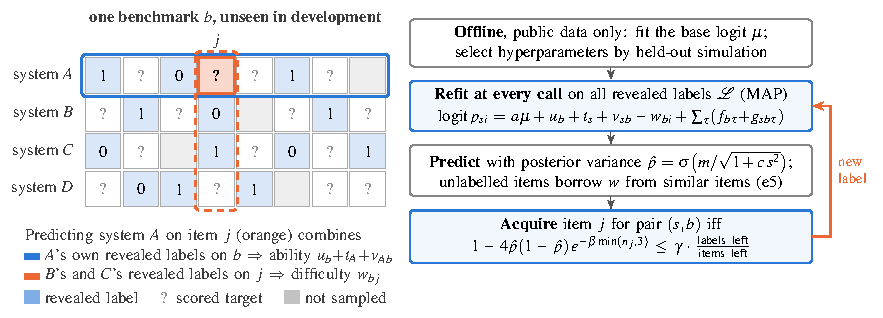
\includegraphics[width=\linewidth]{figs/standalone_overview.pdf}
  \caption{\textbf{Two evidence paths and the pipeline.} \emph{Left:} on a benchmark never seen in development, the prediction for system $A$ on item $j$ combines $A$'s own revealed labels (blue row, which inform its ability) with other systems' revealed labels on the same item (orange column, which inform the item's difficulty). \emph{Right:} public data fit only a base logit and select hyperparameters in simulation. Online, the model is refitted on all revealed labels, predicts with its posterior variance, and the acquisition rule decides which streamed items to reveal.}
  \label{fig:overview}
\end{figure}

%=====================================================================
\section{Task and protocol}\label{sec:task}
%=====================================================================
A \emph{subject} $s$ is a dictionary describing a system (model name, provider, dates, harness, harness version, reasoning effort, free-form features). An \emph{item} $i$ is a dictionary (content, features, interactors, benchmark $b(i)$). The label $y_{si}\in\{0,1\}$ records whether the response was correct, and the target is $p_{si}=\Pr(y_{si}=1)$.
Every sampled pair $(s,b)$ has at least 80 distinct items, which are split at random into an acquisition and an evaluation pool of equal size. All recorded responses of an item stay in the same pool. Between checkpoints, acquisition items arrive one at a time, and \texttt{acquisition\_function(input, prediction, labeled, context)} decides whether to reveal one binary label. The context gives \texttt{labels\_remaining} (out of 31 for the whole run) and \texttt{items\_remaining}.
At each checkpoint $k\in\{0,1,3,7,15,31\}$ (the number of labels acquired per pair), \texttt{predict(input, labeled)} is called for every evaluation target with $\Lb_k$, the labels revealed so far for \emph{all} pairs. Identical inputs reuse one prediction.
The splits are per pair, so an item in $A$'s evaluation pool can be in $B$'s acquisition pool, and revealing $B$'s label on it is within the rules.
The score is the Brier area under the learning curve on a $\log_2(1+k)$ axis,
\begin{equation}\label{eq:alc}
  \ALC = 0.1\,\bar B_0 + 0.2\,(\bar B_1+\bar B_3+\bar B_7+\bar B_{15}) + 0.1\,\bar B_{31},
  \qquad \bar B_k = \frac{1}{|\mathcal P|}\sum_{(s,b)\in\mathcal P} \mathrm{Brier}_{sb}(k),
\end{equation}
where each pair's Brier score averages over all recorded responses of its evaluation items, and pairs carry equal weight. A constant $0.5$ scores $0.25$. The official \emph{Empirical Mean} baseline \citep{paiecbaseline2026} predicts the pair's observed success rate, or $0.5$ without labels.

%=====================================================================
\section{Public data}\label{sec:data}
%=====================================================================
We used the core tables of the public measurement-db \citep{measurementdb2026}. Of 92.6M response rows over 281 benchmarks, 159 benchmarks have binary item-level responses (68.6M responses). The Brier score of a (subject, item) cell with $n$ responses and $k$ successes, $(np^2-2pk+k)/n$, depends only on $(n,k)$, so we aggregate losslessly to 31.8M cells (\cref{app:data}).
\textbf{Within-pair variation dominates.} Across evaluation-eligible pairs, 72\% of the variance of empirical cell success rates lies within pairs, 19\% between benchmarks and 9\% between subjects within a benchmark. The within-pair share includes item difficulty, subject$\times$item interaction and finite-repeat noise.
\textbf{Items are widely shared before sampling.} For 96\% of eligible pairs (pair-weighted), the median item was answered by at least five other subjects, and the median benchmark's subject$\times$item matrix is 92\% dense. This is availability in the public data, not the coverage a sampled draw realises after acquisition. Other entrants report hidden formative draws of about nine pairs, often one per benchmark \citep{brierrabbit2026,doctawho2026}, which we treat as context only.
\textbf{Subject identity needs the full dictionary.} Keying subjects by (name, harness, version, effort) merges at least half of the subjects in 72 of 159 benchmarks. In MMLU, 150 subjects have empty name and harness fields and differ only in \texttt{subject\_features\_extra}. Our package keys subjects by the full dictionary.

%=====================================================================
\section{Method}\label{sec:method}
%=====================================================================
\paragraph{Predictor.}
A prediction for $(s,i)$ on benchmark $b$ draws on three kinds of revealed labels: the pair's own labels (ability on $b$), other systems' labels on $b$ (the benchmark's level), and other systems' labels on item $i$ or on items of the same category (difficulty). Given the revealed cells $\{(s,i,n_{si},k_{si})\}$ in $\Lb_k$, we fit
\begin{equation}\label{eq:model}
  \logit p_{si} \;=\; a\,\mu \;+\; u_{b} \;+\; t_{s} \;+\; v_{sb} \;-\; w_{bi} \;+\; \sum_{\tau\in T(i)} \big(f_{b\tau} + g_{sb\tau}\big),
\end{equation}
with independent zero-mean Gaussian priors on the benchmark level $u_b$, system offset $t_s$, pair offset $v_{sb}$, item difficulty $w_{bi}$ (items are scoped by benchmark), category effect $f_{b\tau}$ and system$\times$category effect $g_{sb\tau}$. Prior scales are in \cref{app:hp}.
$\mu$ is a scalar base logit, the mean logit of the public training data (in simulation, of the training folds), scaled by $a$.
$T(i)$ holds benchmark-scoped categorical tokens: \texttt{key=value} pairs from \texttt{item\_features} and \texttt{interactors} (identifier-like keys removed), coarse format buckets (length, lines, options, code, math), and template tokens (first four and last three words of the text). The term $g_{sb\tau}$ mirrors the ``user$\times$tag accuracy'' features of knowledge-tracing competitions \citep{riiid2021,wang2021eedi}.
Cells enter a binomial likelihood with an effective count cap $n_{\max}$: successes and trials are scaled by $\min(n,n_{\max})/n$.

\paragraph{Inference and prediction.}
We compute the MAP estimate with 12 sweeps of blockwise Newton updates, each using the exact gradient and a diagonal curvature. Updates of multi-membership token effects are damped by the row's token count. The model is refitted whenever the revealed list changes, and the fit is cached within a worker for repeated calls with the same list.
Each effect's posterior variance is approximated by its inverse diagonal curvature (a diagonal Laplace approximation), or by its prior variance if the group has no labels.
Predictions use the probit approximation to the logistic--Gaussian integral \citep{mackay1992}, $\hat p=\sigma\big(m/\sqrt{1+c\,s^2}\big)$, where $m$ and $s^2$ sum the posterior means and variances and $c$ is a tuned variance adjustment. Low-budget predictions therefore stay near $0.5$.
For an item without labels, $w_{bi}$ is borrowed from labelled items of the same benchmark through a sharp \texttt{multilingual-e5-small} embedding kernel \citep{wang2024me5} (\cref{app:hp}).

\paragraph{Acquisition.}
The Fisher information of a Bernoulli label is $p(1-p)$. With labels remaining, we reveal item $j$ for pair $(s,b)$ iff
\begin{equation}\label{eq:acq}
  1 - 4\hat p_{sj}(1-\hat p_{sj})\,e^{-\beta\min(n_j,3)} \;\le\; \gamma\cdot \texttt{labels\_remaining}/\texttt{items\_remaining},
\end{equation}
always once $\texttt{items\_remaining}\le\texttt{labels\_remaining}$, and never once no labels remain. The right-hand side is the remaining labelling rate, so the threshold relaxes when the budget is under-spent, as in budgeted stream-based active learning \citep{fujii2016budgeted}.
$n_j$ counts labels already revealed on item $j$ for \emph{any} system. A first label on an item informs every pair whose evaluation pool contains it, while later labels add less, and the coverage factor encodes this. We use $\gamma=\beta=1$.

\paragraph{Selected configuration.}
The selected package (\texttt{v6}, Codabench submission 1031141) implements \cref{eq:model,eq:acq} without the known-name offset, with embedding propagation, item tokens and the coverage term, and declares the e5 encoder in \texttt{models.txt}. If the encoder cannot be loaded, it falls back to the same model without propagation. \Cref{app:hp} lists the configuration and the package hash.

%=====================================================================
\section{Evaluation methodology}\label{sec:validation}
%=====================================================================
\paragraph{Simulator.}
Our simulator replays the protocol on public data: per-pair 50/50 splits, streamed acquisition with the official context, $\Lb$ spanning all pairs, the six checkpoints, response-weighted Brier and equal pair weights.
An acquisition reveals \emph{one} binary response, drawn once per candidate from the cell's empirical success fraction and shared by all methods. Evaluation cells keep all their responses.
In the main comparison, benchmarks are held out by 5-fold benchmark-level cross-validation: the base logit is fitted on training folds only, and all methods see identical pairs, streams and draws. Intervals resample whole benchmarks (10{,}000 draws).
The same folds were used for development and hyperparameter search, so these are development-set cross-validation results, not an untouched test.
The main runs use an \emph{embedding-free proxy} of \texttt{v6}: the same model with derived text and template tokens, without embedding propagation.

\paragraph{Sampling regimes.}
How the organisers sample systems is not public, so we bracket it with stress tests.
\emph{Standard}: $\le$20 random subjects per benchmark, pools capped at 200 acquisition and 100 evaluation items (\nStd{} pairs, \nbStd{} benchmarks).
\emph{High overlap}: per benchmark, 100 items drawn from the 200 most-answered, and up to 10 subjects that answered all of them (\nHigh{} pairs, \nbHigh{} benchmarks).
\emph{Sparse}: the same construction with one or two subjects per benchmark (\nSpOne{} pairs on \nbSpOne{} benchmarks; \nSpTwo{} pairs on \nbSpTwo{} benchmarks).

\paragraph{Controlled overlap study.}
Separately, we select the \ovNb{} public benchmarks on which ten subjects answered a common set of 100 items, fix one focal subject's split, stream and one-response draws, and add 1, 3 or 9 partner subjects. Acquisition is the evaluator's random rule, so every predictor sees the same trajectory. The base logit is fitted on the other benchmark folds. A replicate repeats the selection with a different seed.

\paragraph{Differences from the hosted evaluator.}
The metric, evidence structure and context are matched. Remaining differences:
(i) the simulator keys items by id, while the package keys them by content, features and interactors, so duplicated inputs pool only in the package;
(ii) simulator runs omit interactor tokens;
(iii) the simulator's acquisition policy refits every 100 labels and omits token effects, while the package refits at every call;
(iv) the main runs omit embedding propagation (\cref{app:sim});
(v) the sampling design is a proxy.
Revealing the whole response cell instead of one response changes the Empirical Mean baseline by 0.0017 ALC in both main regimes, more than several component effects, so all main results use one-response reveals.

\paragraph{Official formative feedback.}
Each official formative evaluation scores a newly sampled hidden subset \citep{paiec2026}. Four uploads of the identical v3 package scored 0.170, 0.192, 0.176 and 0.200 (\cref{app:noise}). Single formative scores therefore cannot rank close variants, and we used them only to check that packages run.

%=====================================================================
\section{Results}\label{sec:results}
%=====================================================================
\begin{figure}[t]
  \centering
  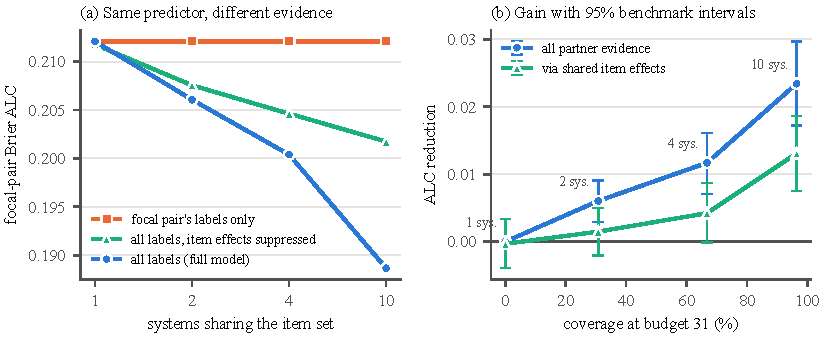
\includegraphics[width=\linewidth]{figs/overlap.pdf}
  \caption{\textbf{Partner evidence helps more as more systems share the items.} Controlled study on \ovNb{} benchmarks where ten systems answered a common set of 100 items. The focal pair's split, stream and reveals are fixed, acquisition is random, and the base logit is held out. \emph{(a)} Focal-pair ALC of the same predictor given only the focal pair's labels, all labels with item effects suppressed, and all labels. \emph{(b)} Paired ALC reductions with benchmark-bootstrap 95\% intervals: from all partner evidence, and the part due to shared item effects. Labels give the number of systems; the x-axis is coverage at budget 31, the share of focal evaluation items revealed for at least one partner.}
  \label{fig:overlap}
\end{figure}

\paragraph{Controlled overlap study.}
\Cref{fig:overlap} isolates cross-system evidence with the predictor held fixed. With one system there is no partner evidence: by construction, the focal-only and all-label predictions coincide (\ovPartOne{}).
With two systems, \ovCovTwo\% of the focal pair's evaluation items have been revealed for the partner by budget 31, and partner evidence improves ALC by \ovPartTwo{} \ovPartCITwo{}.
The gain grows across the tested levels: \ovPartFour{} \ovPartCIFour{} with four systems (\ovCovFour\% coverage) and \ovPartTen{} \ovPartCITen{} with ten (\ovCovTen\%).
Shared item effects account for \ovItemTwo{} \ovItemCITwo{}, \ovItemFour{} \ovItemCIFour{} and \ovItemTen{} \ovItemCITen{} of this, and the remainder comes from the shared benchmark level.
The replicate selection gives \ovPartTenB{} \ovPartCITenB{} and \ovItemTenB{} \ovItemCITenB{} at ten systems.
Prediction alone produces these gains, since acquisition is identical across predictors.

\begin{table}[t]
  \caption{\textbf{Brier ALC in the protocol simulator} (one-response reveals, benchmark-held-out folds; lower is better). Brackets: benchmark-bootstrap 95\% intervals. The model rows are embedding-free proxies; the last row is the selected configuration (\texttt{v6}).}
  \label{tab:main}
  \centering\footnotesize
  \setlength{\tabcolsep}{3pt}
  \begin{tabular}{@{}lllll@{}}
    \toprule
    Method & Standard & High overlap & Sparse, 2 sys. & Sparse, 1 sys. \\
    \midrule
    Constant 0.5                              & 0.2500 & 0.2500 & 0.2500 & 0.2500 \\
    Empirical Mean (official)                 & \aStdEM \ {\scriptsize\ciStdEM} & \aHighEM \ {\scriptsize\ciHighEM} & \aSpTwoEM & \aSpOneEM \\
    Beta(1,1) pair mean                       & \aStdBeta \ {\scriptsize\ciStdBeta} & \aHighBeta \ {\scriptsize\ciHighBeta} & \aSpTwoBeta & \aSpOneBeta \\
    Pair mean shrunk to bench.\ rate          & \aStdEB \ {\scriptsize\ciStdEB} & \aHighEB \ {\scriptsize\ciHighEB} & \aSpTwoEB & \aSpOneEB \\
    \midrule
    Hierarchical model, random acq.           & \aStdHier & \aHighHier & \aSpTwoHier & \aSpOneHier \\
    \quad + uncertainty acquisition           & \aStdHierU & \aHighHierU & \aSpTwoHierU & \aSpOneHierU \\
    \quad + item tokens                       & \aStdTok & \aHighTok & \aSpTwoTok & \aSpOneTok \\
    \quad + coverage term (\texttt{v6} proxy) & \aStdSix \ {\scriptsize\ciStdSix} & \aHighSix \ {\scriptsize\ciHighSix} & \aSpTwoSix & \aSpOneSix \\
    \bottomrule
  \end{tabular}
\end{table}

\paragraph{Main comparison.}
\Cref{tab:main} reports absolute ALC. The benchmark-rate baseline shrinks the pair's own success rate towards the rate of all labels revealed on the benchmark: with $S$ successes in $N$ benchmark labels and $s$ in the pair's own $n$, $p_0=(S+2)/(N+4)$ and $\hat p=(s+2p_0)/(n+2)$.
Much of the gain over the official baseline comes from shrinkage alone. With one label, the Empirical Mean predicts exactly 0 or 1 and scores worse than a constant at budget 1 (\cref{fig:curves}).
Against the strongest shrinkage baseline in each regime, the \texttt{v6} proxy improves ALC by \pStdSixVsEB{} \pciStdSixVsEB{} (standard, benchmark rate), \pHighSixVsEB{} \pciHighSixVsEB{} (high overlap, benchmark rate) and \pSpTwoSixVsBeta{} \pciSpTwoSixVsBeta{} (two systems, Beta).
With a single system per benchmark the comparison with the Beta pair mean is inconclusive (\pSpOneSixVsBeta{} \pciSpOneSixVsBeta{}).

\begin{figure}[t]
  \centering
  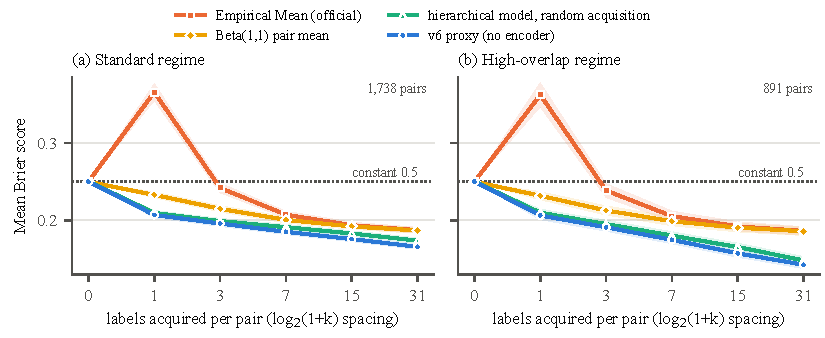
\includegraphics[width=\linewidth]{figs/curves.pdf}
  \caption{\textbf{Brier score at each checkpoint} (mean over pairs; one-response reveals; 1{,}738 pairs in the standard and 891 in the high-overlap regime). Checkpoints are spaced on the official $\log_2(1+k)$ axis. All methods start near the constant reference at budget 0 because the benchmarks are unseen. The Empirical Mean spikes at budget 1, shrinkage (Beta) removes the spike, and the item response model keeps improving as labels accumulate, most strongly with high overlap.}
  \label{fig:curves}
\end{figure}

\begin{table}[t]
  \caption{\textbf{Component effects} (paired ALC differences, negative is better, benchmark-bootstrap 95\% intervals). Each row adds one component to the configuration above it in \cref{tab:main}. ``Active acquisition'' keeps the \texttt{v6}-proxy predictor and compares its acquisition rule with random acquisition.}
  \label{tab:components}
  \centering\footnotesize
  \setlength{\tabcolsep}{4pt}
  \begin{tabular}{@{}lcccc@{}}
    \toprule
    Component & Standard & High overlap & Sparse, 2 sys. & Sparse, 1 sys. \\
    \midrule
    Uncertainty acquisition & \makecell{\dStdUnc\\[-1pt] {\scriptsize\dciStdUnc}} & \makecell{\dHighUnc\\[-1pt] {\scriptsize\dciHighUnc}} & \makecell{\dSpTwoUnc\\[-1pt] {\scriptsize\dciSpTwoUnc}} & \makecell{\dSpOneUnc\\[-1pt] {\scriptsize\dciSpOneUnc}} \\
    Item tokens & \makecell{\dStdTokens\\[-1pt] {\scriptsize\dciStdTokens}} & \makecell{\dHighTokens\\[-1pt] {\scriptsize\dciHighTokens}} & \makecell{\dSpTwoTokens\\[-1pt] {\scriptsize\dciSpTwoTokens}} & \makecell{\dSpOneTokens\\[-1pt] {\scriptsize\dciSpOneTokens}} \\
    Coverage term & \makecell{\dStdCov\\[-1pt] {\scriptsize\dciStdCov}} & \makecell{\dHighCov\\[-1pt] {\scriptsize\dciHighCov}} & \makecell{\dSpTwoCov\\[-1pt] {\scriptsize\dciSpTwoCov}} & \makecell{\dSpOneCov\\[-1pt] {\scriptsize\dciSpOneCov}} \\
    \makecell[l]{Active acquisition\\(\texttt{v6}-proxy predictor)} & \makecell{\dStdAct\\[-1pt] {\scriptsize\dciStdAct}} & \makecell{\dHighAct\\[-1pt] {\scriptsize\dciHighAct}} & \makecell{\dSpTwoAct\\[-1pt] {\scriptsize\dciSpTwoAct}} & \makecell{\dSpOneAct\\[-1pt] {\scriptsize\dciSpOneAct}} \\
    \bottomrule
  \end{tabular}
\end{table}

\paragraph{Which components matter where.}
\Cref{tab:components} separates the additions.
Item tokens help in every regime, including isolated pairs, because category effects are learned from the pair's own labels as well as from others'.
The coverage term needs partners: it helps with high overlap (\dHighCov{} \dciHighCov{}) and leaves decisions unchanged when a benchmark has a single system.
Active acquisition helps when partners exist (\dHighAct{} \dciHighAct{} with high overlap); for isolated pairs the estimate is \dSpOneAct{} \dciSpOneAct{}. Without partner evidence, choosing uncertain items may give a less representative sample of the pair's ability than random choice.
A gate that uses the evaluator's random rule until another system has a label on the benchmark did not help consistently (\cref{app:negative}).

\paragraph{Negative results.}
Several additions did not help (\cref{app:negative}).
The tested cross-benchmark regressions from e5 or Qwen3 embeddings and format features to item easiness or benchmark base rate reached leave-one-benchmark-out $R^2\le0.04$, consistent with evidence that embedding-based difficulty transfers within but not across scenarios \citep{shang2026contextual}. Budget-0 Brier therefore stays near 0.25.
A GBM stacker, per-budget Platt scaling, low-rank skills with benchmark loadings, V-optimal acquisition, an item-discrimination residual, a name$\times$benchmark effect and a two-configuration ensemble were neutral or harmful.
In an offline pilot (NVIDIA API, nine heterogeneous public benchmarks), a 4B open model's difficulty ratings of 450 sampled items had a within-benchmark rank correlation of 0.06. Larger models completed only 35 and 90 ratings under rate limits, too few to interpret.

\paragraph{Official results.}
Thirteen formative runs of nine development packages scored 0.146--0.209, and the four identical v3 runs spanned 0.170--0.200 (\cref{app:noise}). These runs cannot separate small package effects from resampling variability, so we selected \texttt{v6} (submission 1031141, one formative run at 0.209) on the simulator evidence: among the uploaded packages it is the best configuration in both main regimes. Its common-subset summative score is determined by the organisers.

%=====================================================================
\section{Related work}
%=====================================================================
\textbf{IRT and benchmark amortisation.} IRT models \citep{rasch1960,lord1980} compress benchmarks to informative subsets \citep{polo2024tiny}, amortise difficulty calibration from item text \citep{truong2025amortized}, and drive adaptive testing of language models \citep{hofmann2025fluid,krumdick2026}. These items are calibrated on many systems offline, and IRT estimates can be unreliable with few or heterogeneous systems \citep{jiang2026trust}. Our goal is predictive Brier improvement rather than recovery of true latent parameters.
\textbf{Instance-level performance prediction.} Assessors predict per-instance success from system and item features \citep{pacchiardi2025predictaboard,zhou2025adele}, and observational scaling laws predict aggregate scores from low-dimensional abilities \citep{ruan2024observational}. Without benchmark-specific labels, our item-level predictions on unseen benchmarks stay near chance, consistent with \citet{shang2026contextual}.
\textbf{PAIEC entries.} Other public entries also use hierarchical response models for the benchmark-level cold start \citep{doctawho2026,brierrabbit2026}. Our distinct contribution is the fixed-target study of when partner evidence helps, with a sparse boundary and cheap baselines.
\textbf{Adaptive and label-efficient evaluation.} Active testing \citep{kossen2021active,kossen2022ase,berrada2025scaling} and prediction-oriented active learning \citep{bickfordsmith2023epig} select labels for estimation or prediction, and computerised adaptive testing selects by Fisher information \citep{vanderlinden2010,ghosh2021bobcat}. Our rule is a streaming, budget-paced variant with a coverage term for evidence shared across pairs.

%=====================================================================
\section{Limitations and conclusion}
%=====================================================================
\textbf{Limitations.}
The hidden overlap distribution is unknown, and isolated pairs, where partner evidence cannot help, may be common.
The main results use an embedding-free proxy of the package, and repeated responses, duplicated inputs and acquisition-time predictions differ between the simulator and the package (\cref{sec:validation}).
All configurations were chosen on the public benchmark pool that the evaluation folds use.
The controlled study covers \ovNb{} and \ovNbB{} eligible benchmarks (ten complete subjects each) across its two selection seeds.
Text tokens and embeddings ignore images, which matter in about 30 mostly visual public benchmarks, and budget-0 predictions stay near 0.25.

\textbf{Conclusion.}
On benchmarks excluded from development, the revealed labels of other systems on the same items are legitimate evidence. A small test-time item response model turns them into better Brier predictions, with gains that increase with item coverage and vanish for isolated pairs. Shrinkage, item categories and budget-paced acquisition supply the rest. Measuring these effects required a simulator with one-response reveals, strong cheap baselines and benchmark-level intervals, because single formative scores were too noisy to guide the choices.

\paragraph{Reproducibility and disclosures.}
Code and results are released at \url{https://github.com/VaibhavKanojia3773/items-are-shared-paiec}; the same files form the OpenReview supplementary archive, which contains the submitted ZIP, a manifest with full hashes, the simulator, all experiment and figure scripts, the logged outputs behind every table and figure, and instructions (\cref{app:repro}).
Pretrained model: \texttt{intfloat/multilingual-e5-small} (MIT licence), frozen, for item embeddings. Data: the public measurement-db only. No LLM is called at scoring time. The offline rating pilot used open models through the NVIDIA API on public items only and did not influence the submitted method.
Compute: a laptop (12th Gen Intel Core i7-1250U, 16\,GB RAM, no GPU; Python 3.10, NumPy 2.2, pandas 2.3) and cloud notebook sessions with 2$\times$NVIDIA T4 (16\,GB) GPUs, used only to compute embeddings and to run some simulations in parallel. The package needs no GPU. A dictionary-interface replay of 19 public pairs took 65\,s on the laptop CPU without the encoder. Earlier encoder-enabled replays of 24 pairs took 68--93\,s in a cloud notebook session.
The code, experiments and this report were developed with Claude Code (Anthropic) as an AI coding and writing assistant. The author directed the work and checked the claims.

\bibliographystyle{plainnat}
\bibliography{refs}

\appendix
%=====================================================================
\section{Selected configuration}\label{app:hp}
%=====================================================================
\begin{table}[H]
  \caption{\textbf{Selected configuration} (\texttt{v6}, Codabench submission 1031141; full SHA-256 values in \texttt{MANIFEST.md} of the supplement). Values were chosen by random and local search over more than 200 configurations in the standard simulator and checked in the high-overlap regime. A later 202-configuration search over both regimes found no improvement beyond selection noise.}
  \label{tab:hp}
  \centering\footnotesize
  \begin{tabular}{@{}llll@{}}
    \toprule
    Setting & Value & Setting & Value \\
    \midrule
    scale $a$ on $\mu$ & 0.4 & variance adjustment $c$ & 0.1 \\
    $\sigma_u,\ \sigma_t,\ \sigma_v,\ \sigma_w$ & 1.4, 0.5, 1.0, 2.2 & effective count cap $n_{\max}$ & 1 \\
    $\sigma_f,\ \sigma_g$ & 0.7, 0.3 & Newton sweeps & 12 \\
    kernel $\tau_w$, shrinkage $\kappa_w$ & 0.02, 0.3 & acquisition $\gamma$, coverage $\beta$ & 1.0, 1.0 \\
    name-based ability prior & off & name pooling of $t_s$ & off \\
    item key & content+features+interactors & subject key & full dictionary \\
    probability clip & $[0.005, 0.995]$ & encoder & e5-small (118M) \\
    \bottomrule
  \end{tabular}
\end{table}
For an item without labels, embedding propagation sets $\hat w_{bj} = \sum_i k_{ji}\hat w_{bi}/(\kappa_w+\sum_i k_{ji})$ over labelled items $i$ of the same benchmark, with $k_{ji}=\exp((\cos(e_j,e_i)-1)/\tau_w)$, and variance $\sigma_w^2\,\kappa_w/(\kappa_w+\sum_i k_{ji})$. The acquisition rule uses the package's own prediction, including token effects. Predictions are clipped to $[0.005, 0.995]$. A fitted model is reused for every call with an identical revealed list.

%=====================================================================
\section{Simulator details and embedding runs}\label{app:sim}
%=====================================================================
Earlier embedding-enabled runs (whole-cell reveals; standard 1{,}738 pairs, high overlap 891 pairs; run IDs A1, A2) gave the \texttt{v6} configuration 0.1942 and 0.1847, against 0.2438 and 0.2416 for the Empirical Mean.
Removing embedding propagation changed ALC by $-0.0002$ $[-0.0008, +0.0005]$ and $-0.0001$ $[-0.0005, +0.0003]$: a small effect whose intervals span zero, which supports the embedding-free proxies.
Removing tokens cost $+0.0019$ and $+0.0015$. Without tokens, propagation alone was worth $-0.0022$ (standard), so it remains useful on benchmarks with few informative categories. This is separate from the runtime fallback when the encoder cannot load.
The simulator's acquisition policy refits every 100 labels and scores a pair's acquisition pool in one vectorised call. The embedding subset holds at most 10{,}000 items per benchmark (597{,}441 items).
Seeds: pair sampling uses the fold index, streams $100+$fold, and one-response draws $910+$fold. The overlap study uses selection seeds 0 and 1.

%=====================================================================
\section{Public data details}\label{app:data}
%=====================================================================
\begin{table}[H]
  \caption{\textbf{Public training data} (measurement-db core tables, main branch, downloaded 2 November 2026). The left column counts the full release or the binary item-level subset; the right column counts subjects and pairs within that subset, keyed by the full subject dictionary.}
  \label{tab:data}
  \centering\footnotesize
  \begin{tabular}{@{}lr@{\hspace{2.5em}}lr@{}}
    \toprule
    Response rows, all 281 benchmarks & 92.6M & Distinct items with responses & 3.68M \\
    Benchmarks with binary item responses & 159 & Subjects (full dictionary) & 14{,}529 \\
    Binary responses kept & 68.6M & Distinct model names & 674 \\
    Aggregated cells $(s,i,n,k)$ & 31.8M & Eval-eligible pairs ($\ge$80 items) & 12{,}972 \\
    \bottomrule
  \end{tabular}
\end{table}
The variance decomposition uses empirical success rates of eligible cells: benchmark means, subject-within-benchmark means and within-pair residuals.
In the public sample, 7.8\% of targets (pair-weighted) belong to cells with more than one response, and the Brier floor from repeated responses, computed from these empirical cells, is 0.004. Some benchmarks contain identical inputs under different item ids (babilong: 526k ids, 16.9k distinct inputs), which a content-keyed model pools. Interactors are non-empty in six attack or agent benchmarks. The aggregation and EDA scripts are \texttt{scripts/build\_tables.py} and \texttt{scripts/final\_eda.py}.

%=====================================================================
\section{Variability of official formative scores}\label{app:noise}
%=====================================================================
\begin{figure}[H]
  \centering
  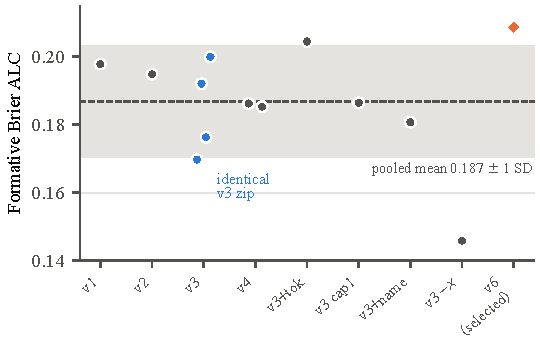
\includegraphics[width=0.62\linewidth]{figs/noise.pdf}
  \caption{\textbf{Official formative scores are single draws of a resampled subset.} Thirteen runs of nine development packages. Four runs of the identical v3 package (blue) span 0.170--0.200; the selected \texttt{v6} run (orange) scored 0.209. The band is the pooled mean $\pm$1 SD, which mixes resampling and package effects.}
  \label{fig:noise}
\end{figure}
The four identical v3 runs have mean 0.184 and sample SD 0.014. Assuming independent draws with this SD, a nominal 95\% interval of half-width 0.005 needs about 30 runs for one package's mean, and about 60 runs per package for the difference between two packages.

%=====================================================================
\section{Negative results}\label{app:negative}
%=====================================================================
\begin{table}[H]
  \caption{\textbf{Ideas that did not help or were not adopted} (development runs with whole-cell reveals unless noted). $\Delta$ is the ALC change against the configuration without the idea (negative is better); other rows report the stated quantity. Run IDs refer to \texttt{logbooks/02\_experiments.md}.}
  \label{tab:negative}
  \centering\footnotesize
  \begin{tabular}{@{}llll@{}}
    \toprule
    Idea & Regime (run) & Quantity & Outcome \\
    \midrule
    kNN text prior of item easiness across benchmarks & standard (E040) & absolute ALC & 0.268 \\
    Ridge: text $\to$ item easiness or benchmark rate & LOBO (X1) & $R^2$ & $\le 0.04$ \\
    GBM stacker on model outputs & standard & $\Delta$ & $+0.0012$ \\
    Per-budget Platt calibration & standard & $\Delta$ & $+0.0003$ \\
    Low-rank skills with benchmark loadings & standard & $\Delta$ & $\ge-0.0001$ \\
    V-optimal acquisition & standard & $\Delta$ & $\approx0$ \\
    Item-discrimination residual & high overlap (F-l5) & $\Delta$ & $\approx0$ \\
    Name$\times$benchmark random effect & both (R5) & $\Delta$ & $\approx0$ \\
    Two-configuration ensemble & high overlap (R5) & $\Delta$ & $+0.0002$ \\
    Qwen3-Embedding-0.6B instead of e5 & standard (E050) & $\Delta$ & $+0.0002$ \\
    Open-LLM difficulty ratings, 4B model & 9 benchmarks (R6) & rank correlation & 0.06 \\
    \midrule
    Known-name ability offset$^{\dagger}$ & high overlap (R7) & $\Delta$ & \dHighName{} {\tiny\dciHighName} \\
    \quad known names only & high overlap (R7) & $\Delta$ & \dHighNameKnown{} {\tiny\dciHighNameKnown} \\
    Overlap gate on acquisition$^{\ddagger}$ & sparse 1 / std.\ (R8) & $\Delta$ & \dSpOneGate{} / \dStdGate{} \\
    & sparse 2 / high (R8) & $\Delta$ & \dSpTwoGate{} / \dHighGate{} \\
    \bottomrule
  \end{tabular}
{\raggedright\footnotesize $^{\dagger}$Adds $a\,\theta_s$ to the base logit, the shrunken mean of benchmark-centred logits of the subject's \texttt{normalized\_name} over public benchmarks ($\theta_s=0$ for unseen names); one-response reveals, embedding-free, benchmark-bootstrap intervals. $^{\ddagger}$Uses the evaluator's random rule until another system has a label on the benchmark; tested with the name offset enabled; all four intervals include zero. Neither is part of the submitted package.\par}
\end{table}

%=====================================================================
\section{Reproduction}\label{app:repro}
%=====================================================================
The repository \url{https://github.com/VaibhavKanojia3773/items-are-shared-paiec} (identical to the supplementary archive) lists every command in \texttt{README.md}.
{\raggedright
\begin{itemize}
  \item \emph{Verify from the release alone} (minutes, no data download): \texttt{paper/scripts/verify\_numbers.py} independently recomputes the reported values; \texttt{paper/scripts/analyze\_r7.py} recomputes every interval and rewrites \texttt{paper/results.tex} from the saved per-pair arrays and the bundled per-row benchmark metadata; the figure scripts redraw \cref{fig:overlap,fig:curves,fig:noise}.
  \item \emph{Recompute from raw data}: \texttt{scripts/download\_core.py} and \texttt{scripts/build\_tables.py} build the 31.8M-cell table; \texttt{paiec/evaluate.py -{}-single -{}-no\_provider -{}-methods \ldots} reproduces \cref{tab:main,tab:components} per regime (\texttt{-{}-formative 100 -{}-rows R}), method suffix \texttt{c1o} gives the gate runs, and \texttt{paiec/overlap.py -{}-seed 0/1} reproduces \cref{fig:overlap}.
  \item \emph{Package}: \texttt{paiec/build\_submission.py} rebuilds an equivalent of the selected ZIP, which passes the official \texttt{check\_submission\_zip.py}.
\end{itemize}
}

\end{document}
